\documentclass[10pt]{article}

\usepackage[margin=1in, letterpaper]{geometry}
\usepackage{parskip}

\usepackage{amsthm, amsmath, amssymb}
\usepackage{gensymb}  % For use of degree symbol
\usepackage[pdftex]{graphicx}
\usepackage{hyperref}

\usepackage{enumerate} % For use of (a), (b), et cetera
\usepackage{booktabs} % Tables
\usepackage[margin=20pt, labelfont=bf, labelsep=period,
justification=justified]{caption} % Captions in figure floats

% ======================
% Document setup, layout
% ======================

% The following metadata will show up in the PDF properties
\hypersetup{
	colorlinks = true,
	urlcolor = magenta,  % Links to URLs
	linkcolor = blue,  % Links within PDF
	pdfauthor = {Aaron Tran},
	pdfkeywords = {berkeley},
	pdftitle = {Astro 121, UG Radio Lab, Lab 3 - \today},
	pdfsubject = {},
	pdfpagemode = UseNone
}

% Don't indent paragraphs
\setlength\parindent{0em}

% Slightly more compact lines
\linespread{0.95}

% ===============
% Useful commands
% ===============
\newcommand {\mt}{\mathrm}
\newcommand {\unit}[1]{\; \mt{#1}}
% http://vemod.net/typesetting-units-in-latex

% Sets, operators
\newcommand {\ints}{\mathbb{Z}}
\newcommand {\ptl}{\partial}
\newcommand {\dl}{\nabla}

\begin{document}

% =======
% Titling
% =======
\begin{center}
\Large{Two-element interferometer fringe measurements at $10.7 \unit{GHz}$}

\normalsize
\textbf{Aaron Tran}${}^{1,2,3}$ \\
Leonardo S. Cassara${}^{1,2}$, Ryan (Xin Xing) Gao${}^{1,2}$, Patrick Kantorski${}^{1,2}$, Salman Kahn${}^{1,4}$ \\
Aaron Parsons${}^{2,5,6}$, Garrett K. Keating${}^{2,5,6}$, Baylee Bordwell${}^{2,6}$ \\
\footnotesize
${}^1$PLSAR Collaboration \\
${}^2$Dept. Astronomy, UC Berkeley, D-23 Hearst Field Annex, Berkeley, CA 94720, USA \\
${}^3$Dept. Earth and Planetary Science, UC Berkeley, 335 McCone Hall, Berkeley, CA 94720, USA \\
${}^4$Dept. Physics, UC Berkeley, 251 LeConte Hall, Berkeley, CA 94720, USA \\
${}^5$Radio Astronomy Laboratory, UC Berkeley, Berkeley, CA 94720, USA \\
${}^6$Undergraduate Radio Laboratory teaching staff \\
\textit{Not received 2014 April 7; submitted 2014 April ??; damnatio memoriae 2014 April ??}
\end{center}

% ========
% Abstract
% ========
\section*{Abstract}

We measure sun and moon angular diameters of $\sim 0.5$--$0.7\degree$ by matching zero crossings in expected modulation functions with fringe envelope curve minima.

\textit{Keywords}: astrometry --- instrumentation: interferometers --- galaxies: individual (NGC 4486) --- ISM: individual (NGC 1976, NGC 6618)

% ============
% Introduction
% ============
\section{Introduction}

Motivation -- measure source declinations and sun moon angular diameters
Pedagogical -- understand interferometry
Least squares fitting to back out meaningful astronomical numbers

Roadmap:
rotation matrices for calculation and ephemerides
Interferometer design
Interferometer signal (averaging, frequency components)
Least squares fitting dec/baseline
Leasts squares fitting diameter
Conclusion

% =================
% Rotation matrices
% =================
\section{Review of astronomical time and coordinates}

We review astronomical timekeeping and coordinate systems used in this study: sidereal time, Julian dates, right ascension and declination, and altitude-azimuth coordinates.
A far more thorough and pedagogical presentation is given by \textit{Green} [1985].
For sanity's sake, I assume the reader is acquainted with geographical and celestial coordinates.

\emph{Julian date} quantifies solar time; a Julian day is $86400 \unit{seconds}$ and a Julian year is $365.25 \unit{days}$.
The timescales used to measure Julian dates may vary (e.g. ephemeris time, terrestrial dynamical time) and are difficult to decipher.
\emph{Sidereal time} quantifies Earth's rotation relative to the fixed stars.
As viewed from Earth, the fixed stars take one \emph{sidereal day} (23h, 56m, 4s of solar time) to sweep out $360\degree$ longitude on the celestial sphere.
A sidereal day is slightly shorter than a solar day due to the Earth's orbital motion around the Sun, and, to a much lesser extent, precession and nutation of the Earth's rotation axis.
\emph{Local sidereal time} (LST) is sidereal time adapted for a specific location (longitude) on Earth, and is defined by the vernal equinox's hour angle (HA).

Astronomical positions are specified by location-agnostic spherical coordinates, typically \emph{right ascension} (RA, $\alpha$) and \emph{declination} (dec, $\delta)$.
To perform observations, we convert $(\alpha, \delta)$ into more useful coordinates for given geographic latitude and longitude -- namely, \emph{altitude} and \emph{azimuth} (alt, az).
Our presentation of the requisite coordinate transformation follows that of Carl Heiles.

Let $(x,y,z)$ specify a right-handed coordinate system where the polar angle is measured relative to the $z$-axis and the azimuth is measured in the $x$-$y$ plane starting from the positive $x$-axis.
In $(\alpha, \delta)$ coordinates, the Earth's rotation axis and equatorial plane correspond to the $z$-axis and $x$-$y$ plane respectively (i.e., right ascension and declination specify a geocentric equatorial coordinate system).
Right ascension is measured counter-clockwise about the $z$-axis starting from the vernal equinox's position on the celestial sphere (positive $x$-axis).
Declination is measured upwards (towards positive $z$) from the equatorial ($x$-$y$) plane.
We see that declination corresponds to the usual polar angle, and right ascension to azimuthal angle.

We compute coordinate transformations using rotation matrices in Cartesian coordinates.
Our coordinate transformations act upon Cartesian coordinate bases from which we measure polar and azimuthal angles for (RA, dec), (HA, dec), and (alt, az) coordinates (e.g., our previously defined $x,y,z$); these transformations are deemed ``passive'' as they only alter the coordinate representations of physical vectors.
A unit vector in $(\alpha, \delta)$ coordinates may be written in Cartesian coordinates as:
\[
	(x, y, z) = (\cos\alpha\cos\delta, \sin\alpha\cos\delta, \sin\delta)
\]
We select a longitude by converting right ascension ($\alpha$) to hour angle (HA):
\[
	\mathrm{HA} = \mathrm{LST} - \alpha
\]
This transformation is a rotation about the $z$-axis and a reflection across the $x$-$z$ plane; (HA, $\delta$) coordinates have reversed handedness compared to $(\alpha, \delta)$ and the rotated $x$-axis is perpendicular to the meridian at which we evaluate LST, HA.
The new coordinate basis has Cartesian representation:
\[
	(x', y', z') = (\cos(\mathrm{HA})\cos\delta, \sin(\mathrm{HA})\cos\delta, \sin\delta)
\]
Two more rotations convert (HA, $\delta$) to (alt, az).
We rotate the $x'$-$z'$ plane by $(\phi - \pi /2)$, where $\phi$ is geographic latitude, then rotate the transformed $x'$-$y'$ plane by $\pi$ radians.
The rotation matrix is constructed as:
\[
	\begin{pmatrix}
		\cos(\pi) & \sin(\pi) & 0 \\
		\sin(\pi) & \cos(\pi) & 0 \\
		0 & 0 & 1
	\end{pmatrix}
	\begin{pmatrix}
		\cos\left(\phi-\pi/2\right) & 0 & \sin\left(\phi-\pi/2\right) \\
		0 & 1 & 0 \\
		\sin\left(\phi-\pi/2\right) & 0 & \cos\left(\phi-\pi/2\right)
	\end{pmatrix}
	=
	\begin{pmatrix}
		-\sin\phi & 0 & \cos\phi \\
		0 & -1 & 0 \\
		\cos\phi & 0 & \sin\phi
	\end{pmatrix}
\]
The final coordinate basis has the same handedness as (HA, $\delta$) coordinates and is written:
\[
	(x'', y'', z'') = (\cos(\mathrm{az})\cos(\mathrm{alt}),
					   \sin(\mathrm{az})\cos(\mathrm{alt}),
					   \sin(\mathrm{alt}))
\]
Altitude is measured upwards from the $x''$-$y''$ plane (i.e., the Earth's local tangent plane) and azimuth is measured clockwise from geographic north.

For arbitrary $(\alpha, \delta)$, the topocentric Cartesian coordinates are:
\begin{equation}
	\hat{s} =
	\begin{pmatrix}
		-\cos(\mathrm{HA}) \sin\phi \cos\delta + \cos\phi \sin\delta \\
		-\sin(\mathrm{HA}) \cos\delta \\
		 \cos(\mathrm{HA}) \cos\phi \cos\delta + \sin\phi \sin\delta
	\end{pmatrix}
\end{equation}

These coordinate transformations correctly predict astronomical positions for both stationary celestial objects and Solar System objects.
Our rotation matrices agree with PyEphem calculations to $\sim 10 \unit{arcseconds}$; note that PyEphem's atmospheric refraction correction must be disabled.
In this study, we use PyEphem to compute all coordinate transformations for observations and data analysis.


% =======
% Methods
% =======
\section{Methods}

% ---------------------
% Interferometer design
% ---------------------
\subsection{Interferometer design}

We measure $10.7 \unit{GHz}$ (X-band) emission using a two-element multiplying interferometer.
The interferometer consists of two antennae (diameter $d \sim 1 \unit{m}$) with east-west baseline $B \approx 10 \unit{m}$ on the rooftop of Wurster Hall, Univ. California Berkeley ($37\degree 52' 12.7'' \unit{N}$, $-122\degree 15' 15.8'' \unit{E}$).
The interferometer beam size is $\lambda/d \sim 1.6\degree$ and angular resolution is $\lambda / B \sim 0.16\degree$.
The stated bandwidth is $10 \unit{MHz}$, though we do not know the antenna response or the frequency band uncertainty of our interferometer dishes.
We conservatively estimate the absolute frequency error to be $\sim 0.1 \unit{GHz}$.

The interferometer may point from $15\degree$ to $87\degree$ in altitude, and its northern field of view is obstructed by a taller portion of Wurster Hall.
We estimate that Wurster Hall obstructs the sky between $-20\degree$ and $10\degree$ azimuth and up to $40\degree$ altitude.
All observations are performed within $17$--$85\degree$ altitude and outside the range of the Wurster Hall obstruction.

A fixed celestial object will move at most $15\degree$ per hour, or $0.125\degree$ every $30 \unit{s}$.
We point the interferometer at $30 \unit{second}$ intervals to keep point sources of interest within $\sim 0.13\degree$ ($10\%$ of interferometer beamwidth) of the interferometer beam's center.
Encoders in the interferometer dishes must be reset (``homed'') every 100 pointings to maintain angular positioning accuracy.
Homing takes $\sim 1 \unit{minute}$ for every $50 \unit{min.}$ of observation.
Interferometer data collected while homing appear as voltage spikes which we  remove during data reduction.

% -----------------
% Signal processing
% -----------------
\subsection{Interferometer signal processing}

The interferometer signal is heterodyne downconverted at the dishes to approximately $1.7 \unit{GHz}$, then to $150 \unit{MHz}$ further along the signal path.
The twice-downconverted signals are mixed and sampled at $\sim 1 \unit{Hz}$.
Amplifiers and filters between downconverting mixers improve signal quality and restrict signal bandwidth to $10 \unit{MHz}$.
But, we necessarily lose information about electric field amplitude at the interferometer dishes.

% ============
% Observations
% ============
\section{Observations}

% Observing campaign
\subsection{Observing campaign}

We observed the Sun, the Moon, and the unresolved point sources NGC 1976 (Orion Nebula, M42), NGC 4486 (Virgo A, M87), and NGC 6618 (Omega Nebula, M17) (Table~\ref{tab:obs}).  The Moon was observed twice: once while waxing crescent with $\sim20\%$ illumination (2014 April 4), and once during a total lunar eclipse (2014 April 15).
All observations are single horizon-to-horizon runs except our observation of the Orion Nebula.

\begin{table}[!ht]
\centering
\caption{Summary of interferometer observations.  Sun and moon flux densities are calculated with $T_b = 14600 \unit{K}$, $217 \unit{K}$ assuming uniform blackbody emission.  Sun brightness temperature is average of estimates for sunspot cycle minima and maxima [\textit{Hafez et al.}, 2014; \textit{Salomonovich and Losovskii}, 1963].}
\label{tab:obs}
\begin{tabular}{@{}rrrr@{}}
    \toprule
    Object & $S_\nu$ (Jy) & Observation start (UT) & Observation end (UT) \\
    \midrule
    Sun & $\sim 4 \cdot 10^6$ & 2014 Apr 01 15:25:44 & 2014 Apr 02 01:02:20 \\
    Moon & $\sim 6 \cdot 10^4$ & 2014 Apr 04 18:54:38 & 2014 Apr 05 06:09:51 \\
    (eclipsed) Moon & $\sim 6 \cdot 10^4$ & 2014 Apr 15 04:09:22 & 2014 Apr 15 12:06:06 \\
    NGC 1976 & $\sim 340$ & 2014 Mar 21 22:53:18 & 2014 Mar 22 09:01:47 \\
    NGC 4486 & $\sim 34$ & 2014 Apr 03 03:03:15 & 2014 Apr 03 12:57:36 \\  % From cut at last pointing
    NGC 6618 & $\sim 500$ & 2014 Apr 05 10:07:34 & 2014 Apr 05 17:04:13 \\
    \bottomrule
\end{tabular}
\end{table}

% --------------
% Data reduction
% --------------
\subsection{Data reduction}

As previously mentioned, dish homing takes $\sim1 \unit{minute}$ and introduces spurious voltage spikes as data collection continues during homing and subsequent re-pointing.  We extract homing start and stop times from automatically generated observing logs and remove all data associated with homing and re-pointing (Figure~\ref{fig:reduction}a).  The interferometer output also carries a fluctuating DC offset ($\Delta V \sim \pm 1 \unit{mV}$) comparable to measured voltages for all sources except the sun; we are unable to explain the cause of this variable offset.  We extract the DC offset signal with a $240 \unit{second}$ wide boxcar filter and subtract the offset from the interferometer output.  Figure~\ref{fig:reduction} plots raw and reduced data for the 2014 April 4 moon observation.

\begin{figure}[!ht]
    \centering
    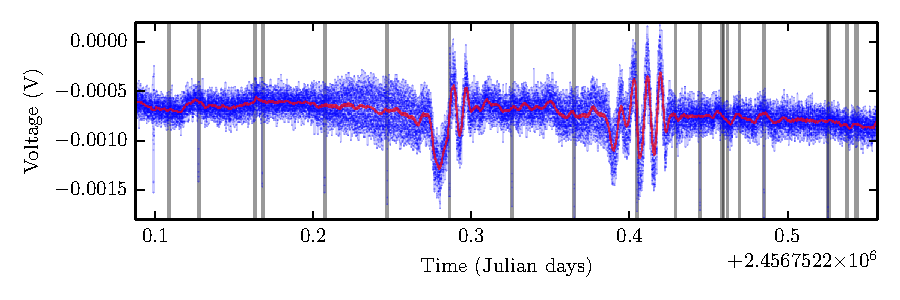
\includegraphics{plots/moon_raw.pdf} \\
    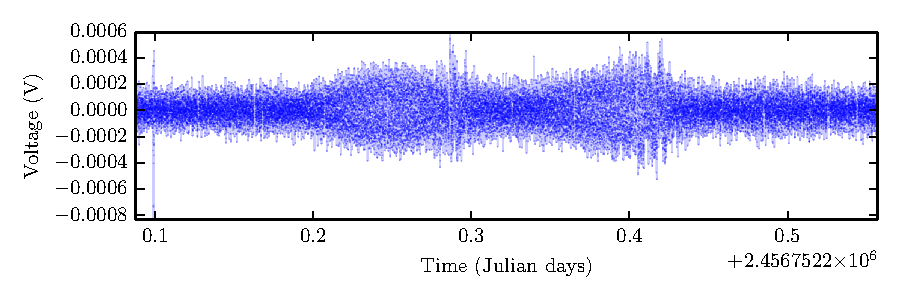
\includegraphics{plots/moon_clean.pdf} \\
    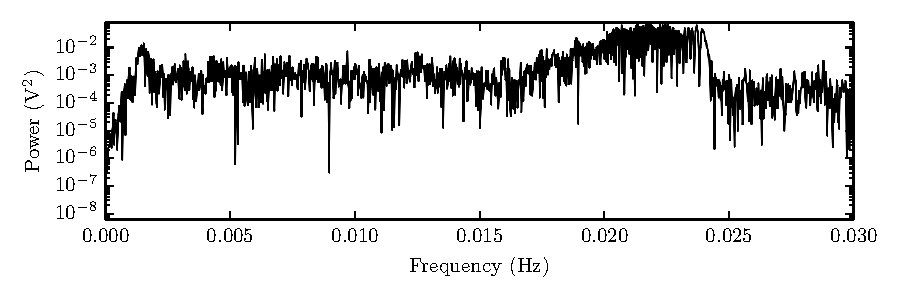
\includegraphics{plots/moon_fft.pdf} \\
    \caption{(top) Raw interferometer output from 2014 April 4 Moon observation; overlaid vertical lines identify homing spikes and gaps in data collection. (middle) Interferometer output with fluctuating DC offset and homing spikes removed.  Data reduction allows fringe modulation to be recovered and extracted.  (bottom) Partial power spectrum of reduced interferometer data.}
    \label{fig:reduction}
\end{figure}

We compute power spectra as a function of frequency from cleaned data using the discrete Fourier transform.  For moon and sun observations, we observe a gradually increasing signal from $0.015$--$0.027 \unit{Hz}$ consistent with the range of expected fringe frequencies; in point source data, a weak and possibly spurious peak may be discerned near $0.027 \unit{Hz}$.  We assume the sampling period is $1 \unit{second}$ despite gaps in data sampling, introducing some error.  Although we do not account for uneven sampling here, we refer the interested reader to work by \textit{Dutt and Rokhlin} [1993] and \textit{Ferraz-Mello} [1981].

% =======
% Results
% =======
\section{Results}

% ---------------------
% Interferometer signal
% ---------------------
\subsection{Interferometer point source response}

The interferometer outputs the product of two voltage signals.  For a point source, the response in time varies as
\begin{align*}
	F(t) &= \cos(2\pi\nu t) \cos\left(2\pi\nu \left[ t + \tau \right] \right) \\
		 &\approx \cos\left(2\pi\nu \tau\right)
\end{align*}
where $\tau = (B_y / c) \cos\delta \sin(h_s) + \tau_c$ considers both geometric and cable delay and we have dropped the sum term which oscillates at $22 \unit{GHz}$.
Then:
\[
	F(t) = \cos(2\pi\nu\tau_c)
			\cos \left[2\pi \left(\frac{B_y}{\lambda}\cos\delta\right)
			           \sin h_s \right]
			- \sin(2\pi\nu\tau_c)
			\sin \left[2\pi \left(\frac{B_y}{\lambda}\cos\delta\right)
			           \sin h_s \right]
\]

% ----------------------
% Dec / baseline fitting
% ----------------------
\subsection{Declination measurement from fringe frequencies}

The fringe frequency for a point source encodes information about the interferometer and source position in the sky.

Brute force least-squares implementation and results.

Frequency/wavelength? Probably 5 to 10 percent error (10.5 to 11.5 GHz).

Error in dec/baseline?

\begin{figure}[!ht]
    \centering
    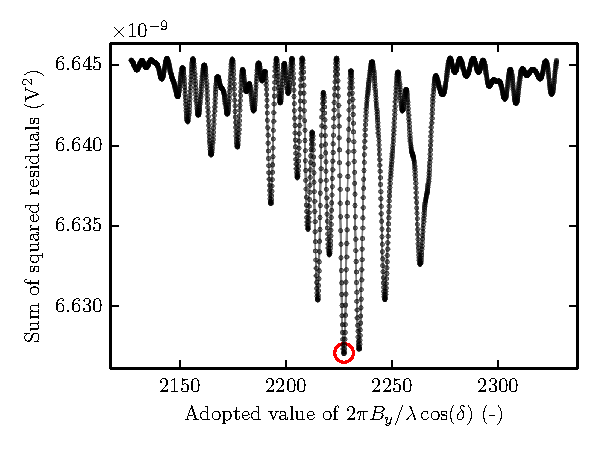
\includegraphics{plots_fitting/orion_dec_fits_lsq.pdf} \\
    \caption{Shitty caption}
\end{figure}

Cable delay is order of 30-40 picoseconds, or about $1 \unit{cm}$.
Note that the maximum measurable cable delay, assuming 11 GHz,
is $91 \unit{ps}$

Declination -- assume $f = 10.7 \pm 0.1 \unit{GHz}$, $B = 10 \pm 0.1 \unit{m}$.

% ----------------
% Diameter fitting
% ----------------
\subsection{Angular diameters of the Sun, Moon}

We now examine the interferometer response to extended sources in the sky, which is proportional to:
$$
    R(h_s) = \int I_\nu (\Delta h) \cos(2\pi\nu \tau_{\mathrm{tot}}) d(\Delta h)
$$
Here $h_s$ is the hour angle of the extended source's center, and $\Delta h = h - h_s$ is hour angle $h$ measured relative to our source.  This is simply the visibility equation with a cosine Fourier transform from our signal mixing, integrated over a 1-D sky.  We may think of this equation as integrating the impulse response over source extent; for $I_\nu(h_s) = \delta(\Delta h)$, we recover the usual fringe response $F(h_s) = \cos(2\pi\nu \tau_{\mathrm{tot}})$.  Conveniently, our antenna beamwidth (response) completely covers all extended sources of interest, namely the Sun and Moon.  To obtain a 1-D intensity distribution, we simply integrate source specific intensity perpendicular to the baseline direction.  For a symmetric source of small angular extent (so that we may Taylor expand in hour angle):
$$
    R(h_s) \approx \cos(2\pi\nu \tau_{\mathrm{tot}}(h_s)) \int I_\nu (\Delta h) \cos(2\pi f_f \Delta h) d(\Delta h)
$$
The left-hand $\cos$ term is simply the point source fringe response; the right-hand integral is a modulation function.  This modulation function should predict our interferometer output's envelope curve (Figure~\ref{fig:sunFringes}).

The modulation function depends on the angular diameter of the source.  Consider a circular source of angular radius $R$ and uniform specific intensity; the source then has 1-D intensity profile $I_\nu(\Delta h) = \frac{1}{R} \left( R^2 - (\Delta h)^2 \right)^{1/2}$.  The corresponding modulation function is:
\begin{align*}
    \mathrm{MF} &= \int \frac{1}{R} \left( R^2 - (\Delta h)^2 \right)^{1/2} \cos(2\pi f_f \Delta h) d(\Delta h) \\
                &\propto \frac{1}{2\pi f_f R} \left(2\pi f_f R\right)
                         \int_0^\pi \sin^2 \theta \cos\left(2\pi f_f R \cos(\theta)\right) d\theta \\
                &\propto \frac{1}{2\pi f_f R} J_1 \left(2\pi f_f R \right)
\end{align*}
where $J_1(z)$ is a Bessel function of the first kind [\textit{Abramowitz and Stegun}, 1964].

\begin{figure}[!ht]
    \centering
    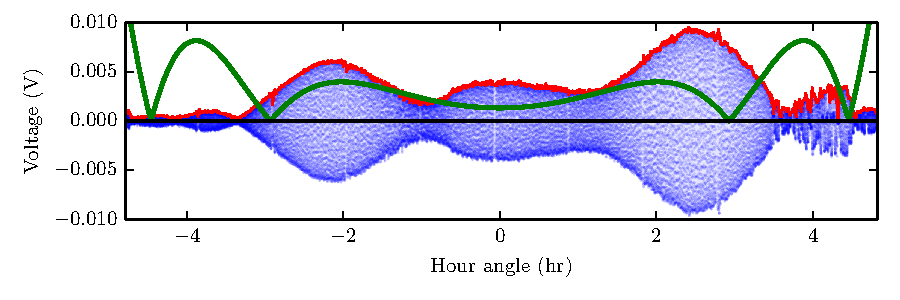
\includegraphics[scale=1]{plots_fitting/sun_fringes_envelopes.pdf} \\
    \caption{Shitty caption}
	\label{fig:sunFringes}
\end{figure}

% ==========
% Discussion
% ==========
\section{Discussion}

It is worth mentioning that finite frequency bandwidth contributes an extra factor of $\mathrm{sinc} (\Delta\nu \tau_{\mt{tot}})$ to the interferometer's extended source response.  For our interferometer, the argument $\Delta\nu\tau < 1$ and so this term has a relatively small effect.

Eclipse observation.

\begin{figure}[!ht]
    \centering
    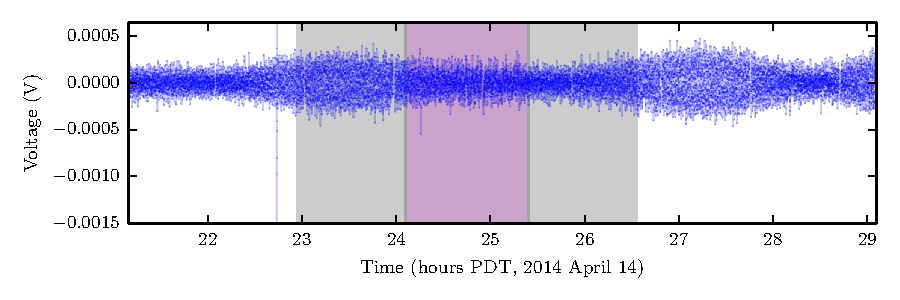
\includegraphics{plots/moon_eclipse_nice_clean.pdf} \\
    \caption{Reduced interferometer data from 2014 April 14 moon observation.  Partial and total eclipse times are highlighted in gray and magenta.}
    \label{fig:eclipse}
\end{figure}

% ===========
% Conclusions
% ===========
\section{Conclusions}



\section{Acknowledgments}

Karto and Baylee's work on the interferometer hardware and software (especially the IDL-Python porting) made this entire lab possible.

\section{Electronic supplement}

All supporting files are stored on the repository:\\
\href{https://github.com/aarontran/ay121}
{https://github.com/aarontran/ay121/lab3/}.

\section{References}

\hangindent 0.25in Condon, J. J. and S. M. Ransom (2006), Essential Radio Astronomy, \\
\href{http://www.cv.nrao.edu/course/astr534/ERA.shtml}
{http://www.cv.nrao.edu/course/astr534/ERA.shtml}.

\hangindent 0.25in Dutt, A. and V. Rokhlin (1993), Fast Fourier transforms for
nonequispaced data, \textit{SIAM J. Sci. Comput.}, \textit{14}(6),
1368--1393, doi:10.1137/0914081.

\hangindent 0.25in Ferraz-Mello, S. (1981), Estimation of periods from
unequally spaced observations, \textit{Astrophys. J.}, \textit{86}(4),
619--624, doi:10.1086/112924.

\hangindent 0.25in Green, R. M. (1985), \textit{Spherical astronomy}, 520pp.,
Cambridge Univ. Press, Cambridge.

\hangindent 0.25in Hafez, Y. A. et al. (2014), A radio determination of the time of the New Moon, \textit{Mon. Not. Roy. Astron. Soc.}, \textit{439}(3), 2271--2280, doi:10.1093/mnras/stt2476.

\hangindent 0.25in Pettit, E. and S. B. Nicholson (1930), Lunar radiation and temperatures, \textit{Astrophys. J.}, \textit{71}, 102--135, doi:10.1086/143236.

\hangindent 0.25in Salomonovich, A. E. and B. Y. Losovskii (1963), Radio-brightness distribution on the lunar disk at 0.8 cm, \textit{Soviet Astron.}, \textit{6}(6), 833--839.

\end{document}